\subsection{Leerlaufspannung und Eigenwiderstand (Messreihe a)}
Am Voltmeter werden der Eingangswiderstand
\begin{equation*}
  R_{V}=\SI{10e6}{\symup{\Omega}}
\end{equation*}
\\und die Leerlaufspannung
\begin{equation*}
  U_{0, Mono., theo}=\SI{1.4}{V}
\end{equation*}
\\abgelesen.

\subsection{Klemmenspannung an der Monozelle (Messreihe b)}
Die Messwerte sind in Tabelle \ref{tab:Mono} aufgeführt.


\begin{table}
  \centering
  \caption{Messdaten}
  \label{tab:some_data}
  \begin{tabular}{c c }
    \toprule
     I &	 U	   \\
     mA &  V  \\
    \midrule
   83  & 0,940	\\
   70  & 1,000	\\
   61  & 1,000	\\
   55  & 1,050	\\
   50  & 1,080	\\
   45  & 1,110	\\
   41  & 1,140	\\
   37  & 1,155	\\
   35  & 1,170	\\
   32  & 1,185	\\
   31  & 1,200 \\
   29  & 1,200 \\
   25  & 1,215	\\
   24  & 1,230	\\

    \bottomrule
  \end{tabular}
\end{table}

Die Klemmenspannung U ist in Abbildung \ref{fig:Mono} gegen den Belastungsstrom I aufgetragen.
\\Die lineare Regression der Form $ax+b$ hat die Parameter:
\begin{align*}
a=& \SI{-5.05722 \pm 0.00003}{\symup\Omega}\\
b=& \SI{1.34431 \pm 0.00006}{V}.\\
\end{align*}
\begin{figure}[h!]
  \centering
  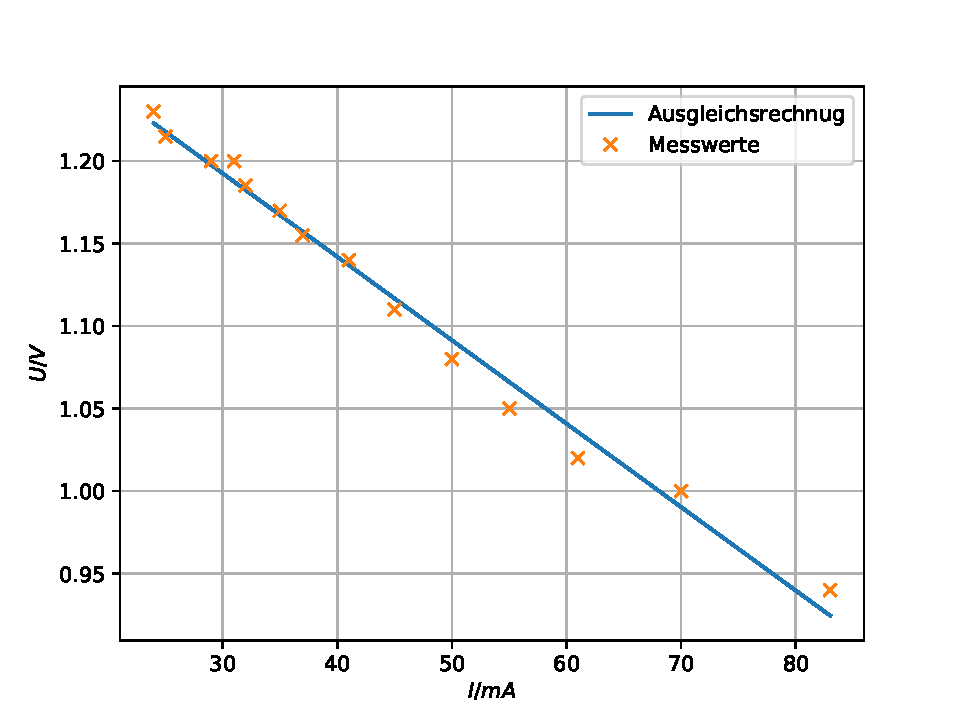
\includegraphics[width=\textwidth]{Mono.pdf}
  \caption{Klemmenspannung U gegen den Belastungsstrom I mit der Monozelle}
  \label{fig:Mono}
\end{figure}
\\Dabei ist nach Gleichung \eqref{eqn:klemme} die Steigung a gleich dem Innenwiderstand und es ergibt sich
\begin{equation*}
  R_{i}=\SI{5.05722 \pm 0.00003}{\symup\Omega}.
\end{equation*}
\\Der y-Achsenabschnitt b ist gleich der Leerlaufspannung $U_{0}$
\begin{equation*}
  U_{0, Mono1, exp}=\SI{1.34431 \pm 0.00006}{V}.
\end{equation*}
\FloatBarrier

\subsection{Klemmenspannung mit der Gegenspannung (Messreihe c)}
In Tabelle \ref{tab:Gegen} sind die Messwerte zur Klemmenspannung mit der Gegenspannung.


\begin{table}[h!]
  \centering
  \caption{Messreihe b}
  \label{tab:Gegen}
  \begin{tabular}{c c }
    \toprule
     I/mA  &	 U/V	   \\
    \midrule
  2,00 & 2,520\\
  1,70 & 2,340\\
  1,40 & 2,160\\
  1,10 & 2,040\\
  1,00 & 1,950\\
  0,90 & 1,920\\
  0,80 & 1,860\\
  0,70 & 1,845\\
  0,65 & 1,800\\
  0,60 & 1,755\\
  0,55 & 1,740\\
  0,50 & 1,710\\
  0,50 & 1,695\\

    \bottomrule
  \end{tabular}
\end{table}

In Abbildung \ref{fig:Gegen} ist die Klemmenspannung gegen den Belastungsstrom I aufgetragen.
\\Die Parameter der linearen Regression der Form $cx+d$ lauten:
\begin{align*}
c=& \SI{529.614 \pm 0.101}{\symup\Omega}\\
d=& \SI{1.443676 \pm 0.000113}{V}.\\
\end{align*}
\begin{figure}[h!]
  \centering
  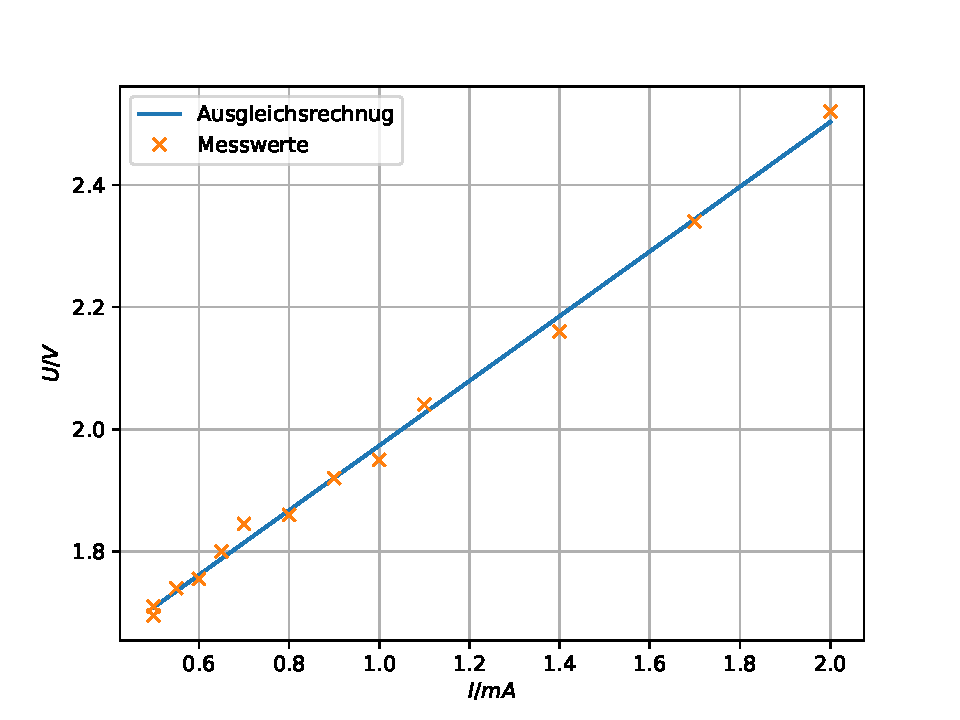
\includegraphics[width=\textwidth]{Gegen.pdf}
  \caption{Klemmenspannung U gegen den Belastungsstrom I an der Monozelle mit der Gegenspannung}
  \label{fig:Gegen}
\end{figure}
\\Die Steigung c der gefitteten Funktion ist der Innenwiderstand:
\begin{equation*}
  R_{i}= \SI{529.614 \pm 0.101}{\symup\Omega}.
\end{equation*}
\\Die Leerlaufspannung ist gleich dem y-Achsenabschnitt d:
\begin{equation*}
  U_{0, Mono2, exp}=\SI{1.443676 \pm 0.000113}{V}
\end{equation*}
\FloatBarrier

\subsection{Klemmenspannung mit der Rechteck- und Sinusspannung (Messreihe d)}
Die Leerlaufspannung wird als
\begin{equation*}
  U_{0, Rechteck, theo}=\SI{0.5}{V}
\end{equation*}
\\gemessen.
\\Zur Schaltung mit der Rechteckspannung werden die Klemmenspannung U und der Belastungsstrom I in Tabelle \ref{tab:Recht} gemessen.


\begin{table}[h!]
  \centering
  \caption{Messreihe c}
  \label{tab:Recht}
  \begin{tabular}{c c }
    \toprule
     I/mA &	 U/V	   \\
    \midrule
   5,9  & 0,155	\\
   5,1  & 0,200	\\
   3,8  & 0,270	\\
   3,1  & 0,300 \\
   2,7  & 0,340 \\
   2,4  & 0,360	\\
   2,1  & 0,380	\\
   1,8  & 0,390	\\
   1,6  & 0,400 \\
   1,5  & 0,410	\\
   1,4  & 0,420	\\


    \bottomrule
  \end{tabular}
\end{table}

Die Messwerte sind in Abbildung \ref{fig:Recht} aufgetragen.
\\Die lineare Regression mit der Funktion $ex+f$ liefert die Parameter:
\begin{align*}
e=& \SI{-58.67 \pm 0.002}{\symup\Omega}\\
f=& \SI{0.497020 \pm 0.000018}{V}.\\
\end{align*}
\begin{figure}[h!]
  \centering
  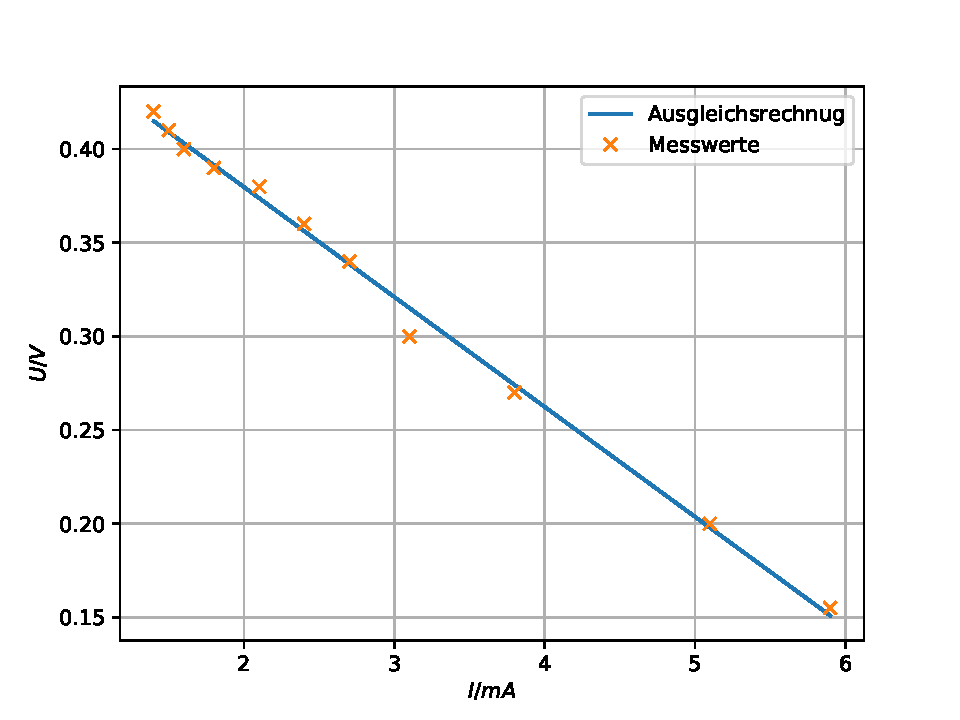
\includegraphics[width=\textwidth]{Recht.pdf}
  \caption{Klemmenspannung U gegen den Belastungsstrom I mit der Rechteckspannung}
  \label{fig:Recht}
\end{figure}
\\Der Innenwiderstand ist nun gleich der Steigung e des Graphen
\begin{equation*}
  R_{i}= \SI{58.67 \pm 0.002}{\symup\Omega}.
\end{equation*}
\\Der y-Achsenabschnitt f beschreibt die Leerlaufspannung:
\begin{equation*}
  U_{0, Rechteck, exp}=\SI{0.497020 \pm 0.000018}{V}.
\end{equation*}
Mit der eingehenden Sinusspannung ist die Leerlaufspannung
\begin{equation*}
  U_{0, Sinus, theo}=\SI{0.67}{V}.
\end{equation*}
\\Es wird erneut die Klemmenspannung U und der Belastungsstrom I gemessen.
Die Messwerte für die Messreihe mit der Sinusspannung sind in Tabelle \ref{tab:Sin} aufgetragen.


\begin{table}[h!]
  \centering
  \caption{Messreihe d}
  \label{tab:Sin}
  \begin{tabular}{c c }
    \toprule
     I/mA &	 U/V	   \\
    \midrule
  0,65  &   0,210\\
  0,47  &   0,330\\
  0,32  &   0,440\\
  0,24  &   0,500\\
  0,18  &   0,530\\
  0,15  &   0,560\\
  0,13  &   0,570\\
  0,11  &   0,580\\
  0,10  &   0,590\\
  0,09  &   0,595\\
  0,08  &   0,600\\


    \bottomrule
  \end{tabular}
\end{table}

In Abbildung \ref{fig:Sin} sind die Messwerte abgebildet.
\\Die Parameter der linearen Regression der Form $gx+h$ sind:
\begin{align*}
g=& \SI{-690.29 \pm 0.05}{\symup\Omega}\\
h=& \SI{0.658594 \pm 0.000004}{V}.\\
\end{align*}
\begin{figure}[h!]
  \centering
  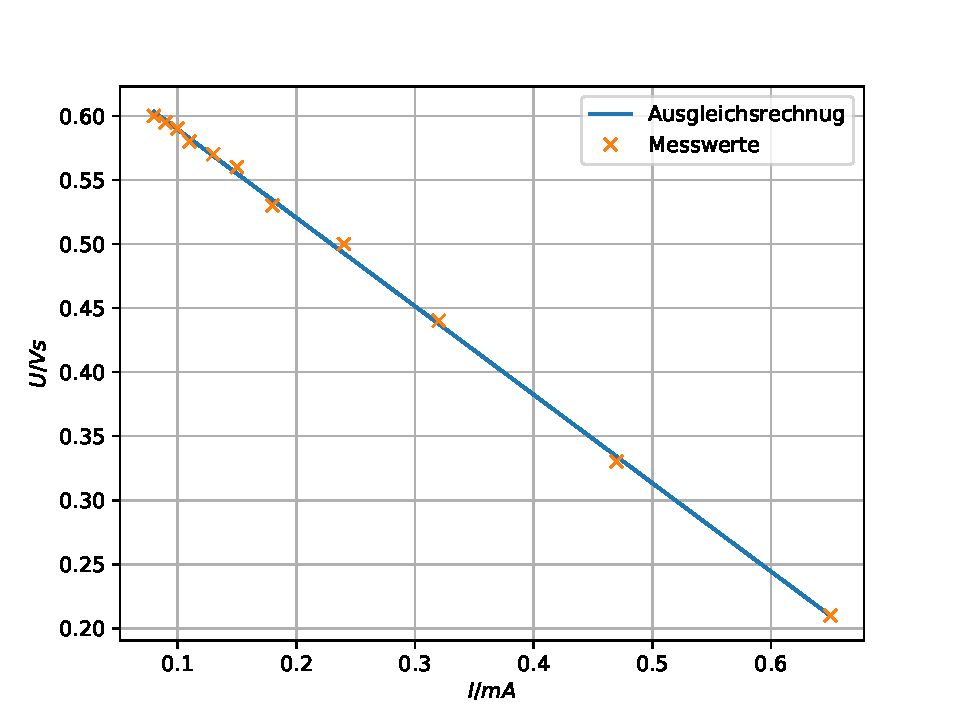
\includegraphics[width=\textwidth]{Sin.pdf}
  \caption{Klemmenspannung U gegen den Belastungsstrom I mit der Sinusspannung}
  \label{fig:Sin}
\end{figure}
\\Bei der Sinusspannung gilt ebenfalls, dass die Steigung g dem Innenwiderstand entspricht:
\begin{equation*}
  R_{i}=\SI{690.29 \pm 0.05}{\symup\Omega}.
\end{equation*}
\\Die Leerlaufspannung wird durch den y-Achsenabschnitt h dargestellt:
\begin{equation*}
  U_{0, Sinus, exp}=\SI{0.658594 \pm 0.000004}{V}.
\end{equation*}
\FloatBarrier

\subsection{Systematischer Fehler der $U_{0}$-Messung (Aufgabe c)}
Zur Berechnung des systematischen Fehlers der Messung der Leerlaufspannung $U_{0}$ wird Formel \eqref{eqn:...} unter Beachtung des hochohmigen Eingangswiderstands des Voltmeters und unter Nutzung des Ohm'schen Gesetzes abgeändert zu:
%U0=IRv+IRi
%U0=I(Rv+Ri)
%U0=Uk/Rv(Rv+Ri)
%U0=Uk(1+Ri/Rv)
\begin{equation}
U_{0} = I \left(R_{V}+R_{i} \right)
      = \frac{U_{K}}{R_{V}} \left( R_{V}+R_{i} \right)
      = U_{K}+U_{K} \frac{R_{i}}{R_{V}}.
\end{equation}
\\Mit
\begin{equation*}
  \frac{R_{i}}{R_{V}}=\SI{5.05722e-7}{}
\end{equation*}
\\ergibt sich ein Fehler der Leerlaufspannung von
\begin{equation*}
  \Delta U_{0}= U_{0, Mono., exp} \cdot \frac{R_{i}}{R_{V}} = \SI{7.080108e-7}{V}
\end{equation*}
\FloatBarrier

\subsection{Systematischer Fehler bei nachgeschaltetem Voltmeter (Aufgabe d)}
Analog zur Rechnung im vorherigen Abschnitt beeinflussen der Innenwiderstand des Voltmeters $R_{i}$ und der Innenwiderstand des Amperemeters $R_{A}$ ebenfalls den Strom- und Spannungsfluss der Schaltung.
%U0=IRv+IRa+IRi
%U0=I(Rv+Ra+Ri)
%U0=Uk/Rv(Rv+Ra+Ri)
%U0=Uk(1+Ra/Rv+Ri/Rv)
Es ergibt sich folglich ein systematischer Fehler der Form
\begin{equation*}
  \Delta U_{0}=U_{K} \left( 1+ \frac{R_{A}}{R_{V}} + \frac{R_{i}}{R_{V}} \right).
\end{equation*}
\FloatBarrier

\subsection{Umgesetzte Leistung (Aufgabe e)}
Die Messwerte zur Messung der Leistung sind in Tabelle \ref{tab:Leistung} eingetragen.
In Abbildung \ref{fig:Leistung} sind die errechnete Leistung $N(R_{a})$ gegen den errechneten Belastungswiderstand $R_{a}$ aufgetragen.
Außerdem ist in der Abbildung die Theoriekurve der Form
\begin{equation*}
  N=\frac{U_{0}^2 R_{a}}{\left(R_{i} + R_{a} \right)^2}.
\end{equation*}
eingezeichet.


\begin{table}[h!]
  \centering
  \caption{Messreihe e}
  \label{tab:Leistung}
  \begin{tabular}{c c c c}
    \toprule
     I/mA  &	 U/V	& $N=U \cdot I$/W  & $R_{a}=\frac{U}{I}/\symup{\Omega}$ \\
    \midrule
   83  & 0,940	&  0,078    & 11,33 \\
   70  & 1,000	&  0,070    & 14,29 \\
   61  & 1,000	&  0,062    & 16,72 \\
   55  & 1,050	&  0,058    & 19,09 \\
   50  & 1,080	&  0,054    & 21,60 \\
   45  & 1,110	&  0,050    & 24,67 \\
   41  & 1,140	&  0,047    & 27,81 \\
   37  & 1,155	&  0,043    & 31,22 \\
   35  & 1,170	&  0,041    & 33,43 \\
   32  & 1,185	&  0,038    & 37,03 \\
   31  & 1,200  &  0,037    & 38,71 \\
   29  & 1,200  &  0,035    & 41,38 \\
   25  & 1,215	&  0,030    & 48,60 \\
   24  & 1,230	&  0,030    & 51,25 \\

    \bottomrule
  \end{tabular}
\end{table}

\begin{figure}[h!]
  \centering
  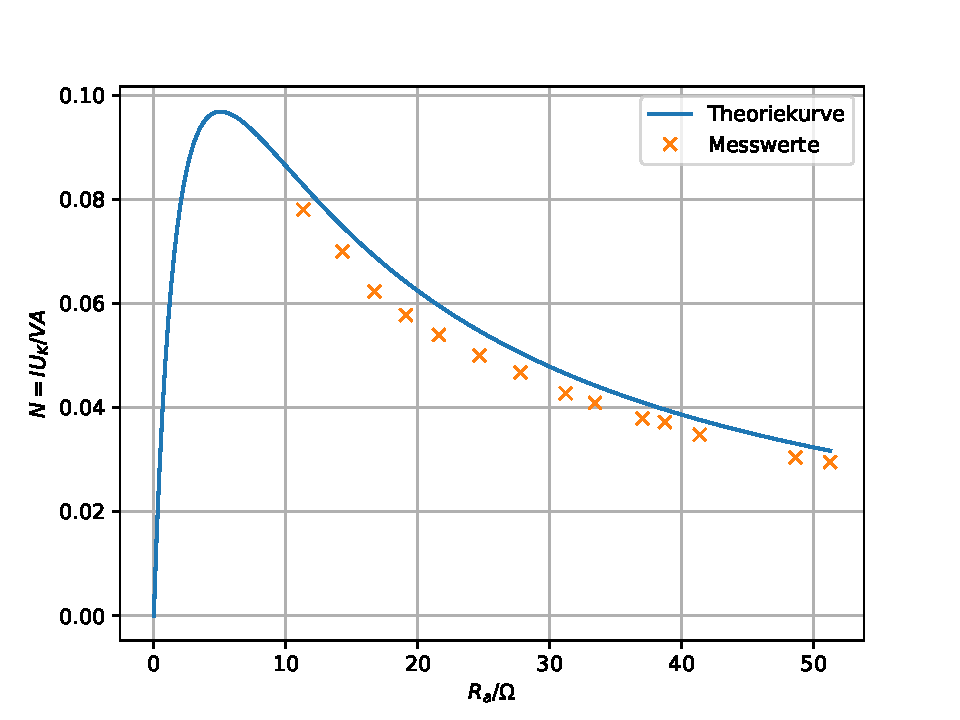
\includegraphics[width=\textwidth]{Leistung.pdf}
  \caption{Leistung N gegen den Belastungswiderstand $R_{a}$}
  \label{fig:Leistung}
\end{figure}
\FloatBarrier
